\section{Implementation}

\subsection{Apps}
Bei Django werden unabhängige Funktionalitäten in unterschiedliche Apps aufgeteilt. Eine App in Django ist eigentlich nichts anderes als ein Python Package, welches eine Reihe von Features zur Verfügung stellt\footcite{django:apps}. Das Ziel dabei ist es, den Code auf die verschiedenen Apps aufzuteilen, so dass diese unabhängig voneinander wiederverwendet werden können.  \\
In der Tabelle \ref{table:django_apps} sind die einzelnen Apps aufgelistet, welche für Aufgaben-Coaching erstellt wurden.

\begin{table}[h]
	\centering
	\begin{tabu} to 0.9\textwidth {l X}
	\toprule
	App & Beschreibung \\ 
	\midrule	
	user & In der Users App befindet sich die gesamte Logik zum erstellen und verwalten der User. \\
	\midrule
		school\_admin & Die school\_admin App ist für die Erstellung von Klassen sowie der Zuweisung von Schülern und Lehrern in Klassen zuständig. \\
	\midrule
	school\_teacher & In dieser App können Lehrer die Fächer für ihre Klasse freischalten und Aufgaben dem Wochenplan hinzufügen. \\
	\midrule
		exercise & Die exercise App stellt um Aufgaben zu erstellen zur Verfügung. Zudem können gelöste Aufgaben von einem Lehrer bewertet werden. \\
	\midrule 
	study\_content & Diese App beinhaltet die Logik zum bereitstellen von Lerninhalten \\
	\midrule	
	forum & In der forum App wird die komplette Logik für das Forum implementiert. \\
	\bottomrule
	\end{tabu}
	\captionof{table}{Apps Beschreibung}
	\label{table:django_apps}
\end{table}

%\subsubsection*{Datenbank}
%
%Werden mehrere Apps erstellt, muss darauf geachtet werden, wie das Domain Model aussieht. Bei Django werden die einzelnen Models direkt in der App hinterlegt. Somit gibt es kein zentrales 
%
%Die Logik kann ohne Probleme in die verschiedenen Apps aufgeteilt werden. Das Problem dabei ist jedoch die Datenbank. In Django ist es best-practise, die benötigten Models jeweils in der entsprechenden App zu implementieren. Da die einzelnen Tabellen aus der Datenbank eine starke Bindung zu den anderen Tabellen haben, geht diese Bindung somit auch auf die Apps über. Dadurch schwindet der Sinn, die Logik in verschiedene Apps aufzuteilen. Es gibt zwei Möglichkeiten, mit diesem Problem umzugehen. Die erste wäre es, alle Apps zu einer grossen zusammenzulegen und die zweite wäre es bei der zu Beginn gewählten Aufteilung zu bleiben und die starke Koppelung hinzunehmen. 

%TODO Weiterschreiben


\subsection{URLs}

\begin{table}[H]
	\centering
	\begin{tabu} to 0.9\textwidth {l X}
	\toprule
		\textbf{URL} & \textbf{Template} \\
	\bottomrule
		/ & subject\_list.html \\
	\bottomrule
		\textbf{user/} \\
		login/ & registration/login.html \\
		logout/ & registration/logged\_out.html \\ 
		profile/ & user/profile.html \\
		<type>/create/ & user/user\_form.html \\ 
		<pk>/update/ & user/user\_form.html \\
		<pk>/delete/ & user/user\_confirm\_delete.html \\
	\midrule
		\textbf{subject/} \\
		<subject>/ & study\_content/topic\_list.html \\
		<subject>/<topic>/ & study\_content/lesson\_list.html \\
		<subject>/<topic>/<pk>/ & study\_content/lesson\_detail.html \\
	\midrule
		\textbf{school\_admin/} \\
		/ & school\_admin/admin\_overview.html \\
		class/create/ & school\_admin/class\_create.html \\
		class/<class\_pk>/update/ & school\_admin/admin\_class\_management.html \\
		class/<class\_pk>/delete/ & school\_admin/class\_confirm\_delete.html \\
	\midrule
		\textbf{exercise/} \\
		create\_help/<pk>/ & exercise/question\_help\_update.html \\
		review/ & exercise/exercise\_review\_list.html \\
		review/<pk>/<user\_pk>/ & exercise/exercise\_review\_detail.html \\
		review/<pk>/<user\_pk>/archive/ & exercise/exercise\_confirm\_archive.html \\
		review/<pk>/<user\_pk>/reject/ & exercise/exercise\_confirm\_reject.html \\
		review/<pk>/<user\_pk>/<answer\_pk>/ & exercise/answer\_review\_form.html \\
		
		<topic>/ & exercise/exercise\_list.html \\
		<topic>/create/ & exercise/exercise\_question\_create.html \\
		<topic>/<pk>/ & exercise/exercise\_detail.html \\
		<topic>/<pk>/update/ & exercise/exercise\_question\_create.html \\
		<topic>/<pk>/delete/ & exercise/exercise\_confirm\_delete.html \\
		<topic>/<pk>/submit/ & exercise/exercise\_confirm\_submit.html \\
		
		<topic>/<pk>/answer/<question\_pk>/ & \\
		<topic>/<pk>/answer/<question\_pk>/create/ & exercise/answer\_form.html \\
		<topic>/<pk>/answer/<question\_pk>/update/ & exercise/answer\_form.html \\
		<topic>/<pk>/answer/<question\_pk>/detail/ & exercise/answer\_detail.html \\ 
	\midrule
		\textbf{statistic/} \\
		/ & statistic/statistic\_subject.html \\
		exercise/<topic>/<class\_id>/ & statistic/statistic\_exercise.html \\
		exercise/<topic>/<exercise>/<class\_id>/ & statistic/statistic\_detail.html \\
		review/<pk>/<user\_pk>/
		ajax/load\_subjects/ & subject\_dropdown\_list\_options.html \\
		ajax/load\_data/ & subject\_load\_data.html \\
	\midrule
		\textbf{error/} \\
	\end{tabu}
	\captionof{table}{URLs}
\end{table}


Django bietet eine simple Möglichkeit an, um zu definieren, welche Seite mit welcher URL aufgerufen werden kann. Wie man im Bild unten sehen kann, wird eine URL in drei, jeweils kommaseparierten, Teilen definiert:

\begin{minipage}{\textwidth}
	\begin{figure}[H]
		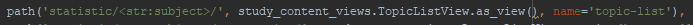
\includegraphics[width=\textwidth, height=\textheight, keepaspectratio]{images/URLBsp.png}
		\caption{URL definition}
	\end{figure}
\end{minipage}


\begin{itemize}
	\itemsep0em
	\item Pfad \\
	Der erste Teil ist der Pfad. Im Beispiel wird der Pfad 'statistic/<str:subject>/' definiert. Das bedeutet, die entsprechende Seite soll über den Pfad ''statistic/'' gefolgt von einem beliebigen Text, in unserem Fall der Titel eines Subjects (zB. Mathematik, Deutsch, etc.), erreichbar sein. 
	\item View \\
	Mit dem zweiten Teil wird definiert, welche View angezeigt werden soll. Im Bild ist es zwar nicht ersichtlich, jedoch werden die Views aus der aktuellen App importiert und können über den Namen ''study\_content\_views'' angesprochen werden. Anschliessend kann über diesen Namen die View angespochen werden, die dargestellt werden soll. In unserem Fall ist dies die View ''TopicListView''.
	\item Name \\
	Im dritten und letzten Teil wird der Pfaddefinition einen Namen gegeben. Dieser Name muss über die ganze Applikation hinweg eindeutig sein und kann dazu verwendet werden, Verlinkungen zwischen den einzelnen Seiten zu definieren. Der Vorteil dabei ist, dass der Pfad sich ändern kann, ohne dass die gemachten Verlinkungen angepasst werden müssen.
\end{itemize}


Es können beliebig viele solcher URLs definiert werden. Das Framework schreibt keine klare Struktur vor. Aus diesem Grund haben wir uns dazu entschieden, die URL Definitionen auf mehere Dateien aufzuteilen und jeweils direkt in den einzlenen Apps abzulegen. Mit diesem Schritt erreicht man mehrere Vorteile. Zum einen wird das Definieren der URLs einiges übersichtlicher und einfacher anzupassen und zum anderen kann man das Risiko von Konflikten zwischen den URLs reduzieren. Schauen wir uns das ganze anhand eines Beispiels an. \\
\begin{minipage}{\textwidth}
	\begin{figure}[H]
		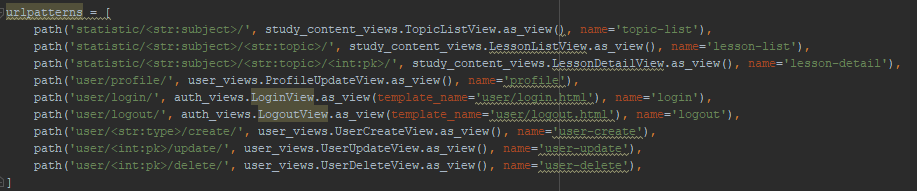
\includegraphics[width=\textwidth, height=\textheight, keepaspectratio]{images/URLschlecht.png}
		\caption{URL Beispiel}
	\end{figure}
\end{minipage}

Im Bild oben sieht man eine kleine Sammlung verschiedener URLs. Bei genauerer Betrachtung fällt auf, dass die URLs von zwei verschiedenen Apps stammen. Die ersten drei URLs gehören zu den Statistiken und die nachfolgenden zur Benutzerverwaltung. Natürlich kann man Vorkehrungen treffen um das ganze übersichtlicher darzustellen, jedoch wird es schwieriger je mehr Definitionen vorliegen. Zum weiteren ist es sehr aufwendig, wenn die URLs angepasst werden sollen. Sollten zum Beispiel die URLs von ''user/...'' auf ''benutzer/...'' geändert werden, muss dies manuell überall angepasst werden. 
Mit unserer Lösung wird diese Datei in drei neue Dateien aufgeteilt und ist danach folgendermassen strukturiert: \\

\textbf{user/urls.py} \\
Diese Datei wird in der App ''user'' abgelegt und kann so zusammen mit der App simpel in eine andere Applikation kopiert und verwendet werden. Im Bild unten werden nun die URLs dargestellt, welche zur Benutzerverwaltung gehören und man kann erkennen, dass die URLs kürzer geworden sind. Das führende ''user/'' wurde entfernt. Wieso das möglich und auch gewünscht ist, wird weiter unten beschrieben. \\
\begin{minipage}{\textwidth}
	\begin{figure}[H]
		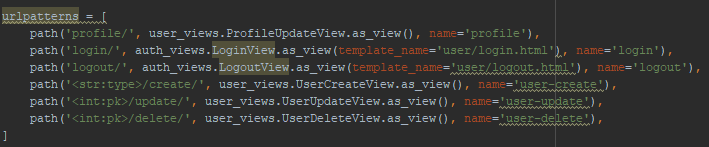
\includegraphics[width=\textwidth, height=\textheight, keepaspectratio]{images/URLuser.png}
		\caption{URL user}
	\end{figure}
\end{minipage}


\textbf{statistic/urls.py} \\
Diese Datei wird in der App ''statistic'' abgelegt. Wie oben das führende ''user/'' entfernt wurde, konnte auch hier auf das führende ''statistic/'' verzichtet werden. \\
\begin{minipage}{\textwidth}
	\begin{figure}[H]
		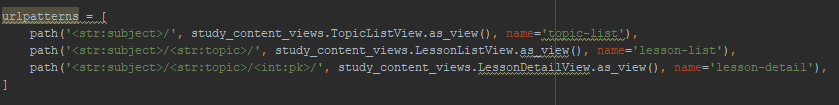
\includegraphics[width=\textwidth, height=\textheight, keepaspectratio]{images/URLstatistic.png}
		\caption{URL statistic}
	\end{figure}
\end{minipage}


\textbf{urls.py} \\
Diese Datei befindet sich in keiner eigenen App, sondern liegt global in der Applikation. Der Inhalt der Datei unterscheidet sich auch gegenüber den andereren Dateien. Hier werden keine URLs definiert, sondern es wird angegeben, wo die definierten URLs abgelegt sind. Oben wurde erwähnt, dass die führenden Pfadelemente (''user/'' und ''statistic/'') weggelassen wurden. Effektiv wurden sie jedoch hierhin verschoben. Sollen nun die URLs der Benutzerverwaltung von ''user/...'' nach ''benutzer/...'' geändert werden, kann dies hier vorgenommen werden und wirkt sich auf alle URLs in der Datei ''user/urls.py'' aus. Nun ist es auch möglich in verschiedenen Apps die selben URLs zu definieren, da sie hier beim einbinden mit dem führenden Pfadelement voneinander unterschieden werden können. Dies kann hilfreich sein, wenn Apps von anderen Entwicklern eingebaut werden würden. \\
\begin{minipage}{\textwidth}
	\begin{figure}[H]
		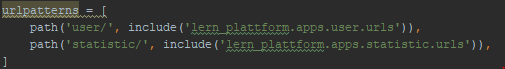
\includegraphics[width=\textwidth, height=\textheight, keepaspectratio]{images/URLglobal.png}
		\caption{URL}
	\end{figure}
\end{minipage}



\subsection{Testing}

Um eine möglichst gute Qualität dieser Arbeit zu gewährleisten, wurde auf folgende Arten von Tests gesetzt:

\begin{itemize}
	\item Unittests \\
		Anhand der Unittests werden die definierten Models getestet. Hierbei wird vorallem Wert darauf gelegt, dass die Models so reagieren, wie sie reagieren sollten. Es soll also zum Beispiel sichergestellt werden, dass ein Objekt als String so repräsentiert wird, wie es erwartet wird. Zusätzlich soll getestet werden, dass nicht mehrere gleiche Objekte erstellt werden können. Wenn in der Datenbank bereits ein Subject mit dem Titel ''Mathematik'' existiert, soll sichergestellt werden, dass kein weiteres erstellt werden kann.
		
	\item Integration Tests \\
		Mit den Integration Tests wird sichergestellt, dass die implementierten Views so arbeiten und reagieren, wie sie sollen. Da die Applikation von drei verschiedenen Benutzergruppen verwendet wird, wurde besonders grossen Wert darauf gelegt zu prüfen, dass jeder Nutzer nur im Rahmen seiner vorbestimmten Rechte agieren kann. Es soll einem Schüler also nicht möglich sein, abgegebene Aufgaben zu bewerten.
		
	\item Usability Tests \\
		Anhand der Usability Tests soll sichergestellt werden, dass das gewählte Design bei den Mockups einfach und selbsterklärend ist. Hierfür wurden den Testusern einige Aufgaben sowie die erstellen Mockups vorgelegt und darauf geachtet, wie sie sich zurecht fanden.
\end{itemize}


\subsubsection*{Usability Tests}
Die Usability Tests wurden basierend auf den in der Planung erstellen Mockups durchgeführt. Die Mockups wurden mit der Webapplikation Balsamiq erstellt \footcite{balsamiq_mockups}.



Um möglichst realitätsgetreue Tests durchzuführen, wurden die Probanden gebeten, die Usability Tests dreimal durchzuführen. Bei jeder Durchführung sollen sie eine andere Rolle einnehmen und andere Aufgaben lösen. Um zu verhindern, oder zumindest die Verfälschung der Tests zu minieren, welche durch das gesammelte Wissen vorheriger Durchführungen entstehen kann, wurden die zugwiesenen Rollen pro Proband in einer unterschiedlichen Reihenfolge zugweisen. In der Tabelle \ref{Usability Test Rollen} ist ersichtlich, dass drei Probanden die Tests durchgeführt haben und welche Rolle sie bei welcher Durchführung zugewiesen bekommen haben. \\

\begin{table}[h]
	\centering
	\begin{tabu} to 0.9\textwidth {l X X X}
	\toprule
		Proband & Durchführung 1 & Durchführung 2 & Durchführung 3 \\ 
	\midrule
		Proband 1 & Schüler & Lehrer & Administrator \\
		Proband 2 & Lehrer & Administrator & Schüler \\
		Proband 3 & Administrator & Schüler & Lehrer \\
	\bottomrule
	\end{tabu}
	\captionof{table}{Usability Test Rollen}
	\label{Usability Test Rollen}
\end{table}






Schüler: \\
\begin{itemize}
	\item asdsa
	\item asd
\end{itemize}



%Das Testen einer Webseite ist eine komplexe Aufgabe, da eine Webseite aus mehreren Schichten unterschiedlicher Logik aufgebaut ist. Das geht von HTTP-Requests über die Validierung von Formularen bis hin zum Rendern von Templates. Mit dem Django-Test-Framework ist es möglich, HTTP-Requests zu simulieren, Testdaten einzufügen, den Output der Applikation zu inspizieren und im allgmeinen zu prüfen, dass der geschriebene Code das tut, was er tun soll.

\subsubsection*{Datenbank}
%Damit die Tests nicht von bereits vorhanden Daten in der Datenbank beeinflusst werden, wird für jeden Testdurchlauf eine eigene temporäre Datenbank erstellt, die exakt wie die in der Produktion verwendete Datenbank konfiguriert ist. Diese temporäre Datenbank wird nach der Testdurchführung wieder vom System entfernt.

\subsubsection*{Test Client}
%Der Test-Client ist eine Pythonklasse, welche als einfacher Webbrowser dient. Mit ihm kann man auf Applikationsebene mit den erstellten Django-Apps agieren. Das heisst, man kann gut und einfach GET und POST Requests simulieren und kann den Inhalt der Webseite überprüfen. 